\documentclass{article}

\usepackage[UTF8, scheme = plain]{ctex}
\usepackage{fancyhdr}
\usepackage{extramarks}
\usepackage{amsmath}
\usepackage{amsthm}
\usepackage{amsfonts}
\usepackage{tikz}
\usepackage[plain]{algorithm}
\usepackage{algpseudocode}
\usepackage{color}
\usepackage{listings}
\usepackage{fontspec}

% \newfontfamily\menlo{Menlo}
\newfontfamily\menlo{Consolas}
\lstset{
    columns=fixed,       
    numbers=left,                                        % 在左侧显示行号
    numberstyle=\tiny\color{gray},                       % 设定行号格式
    frame=none,                                          % 不显示背景边框
    backgroundcolor=\color[RGB]{245,245,244},            % 设定背景颜色
    keywordstyle=\color[RGB]{40,40,255},                 % 设定关键字颜色
    numberstyle=\footnotesize\color{darkgray},           
    commentstyle=\it\color[RGB]{0,96,96},                % 设置代码注释的格式
    stringstyle=\rmfamily\slshape\color[RGB]{128,0,0},   % 设置字符串格式
    showstringspaces=true,                              % 不显示字符串中的空格
    numberstyle=\small\menlo,
    basicstyle=\small\menlo,
    breaklines=true,
}

% \lstset{
%     language=Octave,                % the language of the code
%     basicstyle=\footnotesize,           % the size of the fonts that are used for the code
%     numbers=left,                   % where to put the line-numbers
%     numberstyle=\tiny\color{gray},  % the style that is used for the line-numbers
%     stepnumber=1,                   % the step between two line-numbers. If it's 1, each line 
%                                     % will be numbered
%     numbersep=5pt,                  % how far the line-numbers are from the code
%     backgroundcolor=\color{white},      % choose the background color. You must add \usepackage{color}
%     showspaces=false,               % show spaces adding particular underscores
%     showstringspaces=false,         % underline spaces within strings
%     showtabs=false,                 % show tabs within strings adding particular underscores
%     frame=single,                   % adds a frame around the code
%     rulecolor=\color{black},        % if not set, the frame-color may be changed on line-breaks within not-black text (e.g. commens (green here))
%     tabsize=2,                      % sets default tabsize to 2 spaces
%     captionpos=b,                   % sets the caption-position to bottom
%     breaklines=true,                % sets automatic line breaking
%     breakatwhitespace=false,        % sets if automatic breaks should only happen at whitespace
%     title=\lstname,                 % show the filename of files included with \lstinputlisting;
%                                     % also try caption instead of title
%     keywordstyle=\color{blue},          % keyword style
%     commentstyle=\color{dkgreen},       % comment style
%     stringstyle=\color{mauve},         % string literal style
%     escapeinside={\%*}{*)},            % if you want to add LaTeX within your code
%     morekeywords={*,...}               % if you want to add more keywords to the set
% }

\usetikzlibrary{automata,positioning}

%
% Basic Document Settings
%
%%% page layout
\topmargin=-0.45in
\evensidemargin=0in
\oddsidemargin=0in
\textwidth=6.5in
\textheight=9.0in
\headsep=0.25in

\linespread{1.1}    %%% line spacing

\definecolor{ustcblue}{cmyk}{1,0.8,0,0}

\pagestyle{fancy}
\lhead{\hmwkAuthorName}
\chead{\hmwkClass\ (\hmwkClassInstructor): \hmwkTitle}
\rhead{}
\lfoot{}
\cfoot{\thepage}

\renewcommand\headrulewidth{0.4pt}
\renewcommand\footrulewidth{0.4pt}

\setlength\parindent{0pt}

%
% Create Problem Sections
%

\newcommand{\enterProblemHeader}[1]{
    \nobreak\extramarks{}{Problem \arabic{#1} continued on next page\ldots}\nobreak{}
    \nobreak\extramarks{Problem \arabic{#1} (continued)}{Problem \arabic{#1} continued on next page\ldots}\nobreak{}
}

\newcommand{\exitProblemHeader}[1]{
    \nobreak\extramarks{Problem \arabic{#1} (continued)}{Problem \arabic{#1} continued on next page\ldots}\nobreak{}
    \stepcounter{#1}
    \nobreak\extramarks{Problem \arabic{#1}}{}\nobreak{}
}

\setcounter{secnumdepth}{0}
\newcounter{partCounter}
\newcounter{homeworkProblemCounter}
\setcounter{homeworkProblemCounter}{1}
\nobreak\extramarks{Problem \arabic{homeworkProblemCounter}}{}\nobreak{}

%
% Homework Problem Environment
%
% This environment takes an optional argument. When given, it will adjust the
% problem counter. This is useful for when the problems given for your
% assignment aren't sequential. See the last 3 problems of this template for an
% example.
%
\newenvironment{homeworkProblem}[1][-1]{
    \ifnum#1>0
        \setcounter{homeworkProblemCounter}{#1}
    \fi
    \subsection{Exercise \arabic{homeworkProblemCounter}}
    \setcounter{partCounter}{1}
    \enterProblemHeader{homeworkProblemCounter}
}{
    \exitProblemHeader{homeworkProblemCounter}
}

%
% Homework Details
%   - Title
%   - Due date
%   - Class
%   - Section/Time
%   - Instructor
%   - Author
%

\newcommand{\hmwkTitle}{Homework\ \#2}
\newcommand{\hmwkDueDate}{\today}
\newcommand{\hmwkClass}{Solid Mechanics}
\newcommand{\hmwkClassInstructor}{Professor Z. Wu}
\newcommand{\hmwkAuthorName}{\textbf{Jintao Li}}
\newcommand{\hmwkAuthorID}{\textbf{SA20007037}}
\newcommand{\hmwkAuthoremail}{\textbf{E-mail: lijintao@mail.ustc.edu.cn}}

%
% Title Page
%

% \title{
%     \vspace{2in}
%     \textbf{\hmwkClass:\ \hmwkTitle}\\
%     \normalsize\vspace{0.2in}\large{\hmwkDueDate}\\
%     \vspace{0.2in}\large{\textit{\hmwkClassInstructor}}
%     \vspace{3in}
% }

% \author{\hmwkAuthorName \\
% \hmwkAuthorID}
% \date{}

\renewcommand{\part}[1]{\textbf{ \\ (\alph{partCounter})  }\stepcounter{partCounter} }

%
% Various Helper Commands
%

% Useful for algorithms
\newcommand{\alg}[1]{\textsc{\bfseries \footnotesize #1}}

% For derivatives
\newcommand{\deriv}[1]{\frac{\mathrm{d}}{\mathrm{d}x} (#1)}

% For partial derivatives
\newcommand{\pderiv}[2]{\frac{\partial}{\partial #1} (#2)}

% Integral dx
\newcommand{\dx}{\mathrm{d}x}

% Alias for the Solution section header
\newcommand{\solution}{\textbf{\large \\ Solution: \\}}

% Probability commands: Expectation, Variance, Covariance, Bias
\newcommand{\E}{\mathrm{E}}
\newcommand{\Var}{\mathrm{Var}}
\newcommand{\Cov}{\mathrm{Cov}}
\newcommand{\Bias}{\mathrm{Bias}}

%
\newcommand{\mb}[1]{\mathbf{#1}}

\begin{document}

\begin{titlepage}

\begin{center}

\textcolor{ustcblue}{\includegraphics[width=0.25\textwidth]{./ustc_logo_fig.pdf} \\ [1cm]}
% Title
{ \Huge \bfseries \hmwkClass\ \hmwkTitle}\\[1cm]

\large \textbf{\hmwkClassInstructor} \\ [5cm]

\large \hmwkAuthorName \\ [0.25cm]
\large \hmwkAuthorID \\ [0.25cm]
\large \hmwkAuthoremail
\vfill
% Bottom of the page
{\large November 15, 2020}

\end{center}

\end{titlepage}

\begin{center}
\section{Chapter 2 应变分析}
\end{center}

\begin{homeworkProblem}
求给定区域的平面主应变的大小和方向,如下图所示,
\begin{figure}[h]
    \centering
    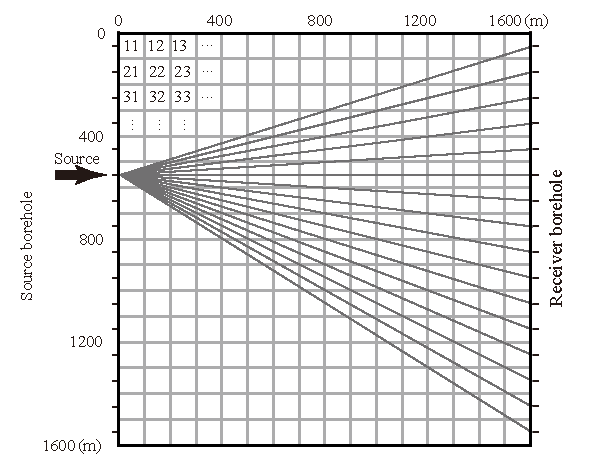
\includegraphics[width=2in, keepaspectratio]{hw2/prob.pdf}
    \label{fig:pro}
\end{figure}

已知相对于参考点(在左下),测点的坐标(单位为km)分别为:

\begin{equation}
    \begin{aligned}
        & G_{11} : (22.06342,  40.58706); \\
        & G_{13} : (23.14246,  33.03411); \\
        & G_{20} : (29.33004,  40.33619).
    \end{aligned}
\end{equation}

测线长度的年度变化(单位为m),见下表。
\begin{table}[h]
    \centering
    \label{tab:tab1}
    \begin{tabular}{|c|c|c|}
    \hline
    基线名称 & 2003年边长 & 2004年边长 \\ \hline
    G20-G13 & 9579.5050 & 9579.5230 \\ \hline
    G20-G11 & 7278.5936 & 7278.6129 \\ \hline
    G13-G11 & 7618.7608 & 7618.7675 \\ 
    \hline
    \end{tabular}
\end{table}

步骤: \\
1. 求三角形的中心坐标;\\
2. 求三条边的方向角度(比如相对于方向东的角度);\\
3. 求三条边上的线应变;\\
4. 根据应变花的方法,求出主应变和主方向;\\
5. 将求得的主方向的角度转化成以北方向为0度来表示。\\

\solution

1. 求三角形的中心点坐标;

\begin{equation}
    \begin{aligned}
    \frac{1}{3} \times (22.06342 + 23.14246 + 29.33004) = 24.64531 \\
    \frac{1}{3} \times (40.58706 + 33.03411 + 40.33619) = 37.62545
    \end{aligned}
\end{equation}
所以中心点的坐标为 $(24.64531, 37.62545)$。

\pagebreak

2. 求三条边的方向角度(比如相对于方向东的角度);

\begin{equation}
    \begin{aligned}
        & G_{11} \rightarrow G_{13} : \theta_1 = 
        \arctan \frac{40.58706-33.03411}{22.06342-23.14246} \approx -1.4289 = -81.87^\circ \\
        & G_{11} \rightarrow G_{20} : \theta_2 = 
        \arctan \frac{40.58706-40.33619}{22.06342-29.33004} \approx -0.0346 = -1.98^\circ \\
        & G_{13} \rightarrow G_{20} : \theta_3 = 
        \arctan \frac{33.03411-40.33619}{23.14246-29.33004} \approx 0.8678 = 49.72^\circ \\
    \end{aligned}
\end{equation} \\

3. 求三条边上的线应变;

\begin{equation}
    \begin{aligned}
        & \epsilon = \frac{\partial u}{\partial x} = \frac{x_2 - x_1}{x_1} \\
        & G_{11} \rightarrow G_{13} : \epsilon_1 = 
        \frac{7618.7675-7618.7608}{7618.7608} = 8.79 \times 10^{-7} \\
        & G_{11} \rightarrow G_{20} : \epsilon_2 = 
        \frac{7278.6129-7278.5936}{7278.5936} = 2.65 \times 10^{-6} \\
        & G_{13} \rightarrow G_{20} : \epsilon_3 = 
        \frac{9579.5230-9579.5050}{9579.5050} = 1.88 \times 10^{-6}
    \end{aligned}
\end{equation} \\

4. 根据应变花的方法,求出主应变和主方向;\\
根据教材第36页的公式,设最大主应力方向为$\sigma_1, \sigma_2$,
与东方向的夹角为 $\alpha$ (与应变方向观测一致)
\begin{equation}
    \begin{aligned}
        & \epsilon_1 = \frac{1}{2}(\sigma_1 + \sigma_2) + 
        \frac{1}{2}(\sigma_1 - \sigma_2)\cos2(\theta_1 - \alpha) \\
        & \epsilon_2 = \frac{1}{2}(\sigma_1 + \sigma_2) + 
        \frac{1}{2}(\sigma_1 - \sigma_2)\cos2(\theta_2 - \alpha) \\
        & \epsilon_3 = \frac{1}{2}(\sigma_1 + \sigma_2) + 
        \frac{1}{2}(\sigma_1 - \sigma_2)\cos2(\theta_3 - \alpha) 
    \end{aligned}
\end{equation}

将第3步得到的$\epsilon_1, \epsilon_2, \epsilon_3, \theta_1, \theta_2, \theta_3$
代入上面的公式中,可以解出:
\begin{equation}
    \sigma_1 = 2.7 \times 10^{-6}, \sigma_2 = 8.79 \times 10^{-7}, \alpha = 7.52^\circ.
\end{equation} 

\textbf{matlab code}
\begin{lstlisting}[language={matlab}]
clear;clc;
syms sigma_1 sigma_2 alpha;
eq1 = 0.5*(sigma_1+sigma_2)+0.5*(sigma_1-sigma_2)*cos(2*(-1.4289-alpha))==8.79e-7;
eq2 = 0.5*(sigma_1+sigma_2)+0.5*(sigma_1-sigma_2)*cos(2*(-0.0346-alpha))==2.65e-6;
eq3 = 0.5*(sigma_1+sigma_2)+0.5*(sigma_1-sigma_2)*cos(2*(0.8678-alpha))==1.88e-6;

[sigma_1, sigma_2, alpha] = solve(eq1, eq2, eq3, sigma_1, sigma_2, alpha);
sigma_1 = single(sigma_1)
sigma_2 = single(sigma_2)
alpha = rad2deg(single(alpha))
\end{lstlisting}


5. 将求得的主方向的角度转化成以北方向为0度来表示;\\
显然,
\begin{equation}
    \alpha^{'} = 90^\circ - \alpha = 82.48^\circ.
\end{equation}





\end{homeworkProblem}

\end{document}